%% Простая презентация с примером включения программного кода и
%% пошаговых спецэффектов
\documentclass[aspectratio=169]{beamer}
\usetheme{SPbAU}
%\useoutertheme{infolines}
\usepackage{fontspec}
\usepackage{xunicode}
\usepackage{xltxtra}
\usepackage{xecyr}
\usepackage{hyperref}
\setmainfont[Mapping=tex-text]{DejaVu Serif}
\setsansfont[Mapping=tex-text]{DejaVu Sans}
\setmonofont[Mapping=tex-text]{DejaVu Sans Mono}
\usepackage{polyglossia}
\setdefaultlanguage{russian}
\usepackage{graphicx}
\usepackage[outputdir=out]{minted}
\usepackage{multicol}
\usepackage{listings}
\setminted[c++]{
  linenos=true,
  fontsize=\footnotesize
}
\lstdefinestyle{mycode}{
  belowcaptionskip=1\baselineskip,
  breaklines=true,
  xleftmargin=\parindent,
  showstringspaces=false,
  basicstyle=\footnotesize\ttfamily,
  keywordstyle=\bfseries,
  commentstyle=\itshape\color{gray!40!black},
  stringstyle=\color{red},
  numbers=left,
  numbersep=5pt,
  numberstyle=\tiny\color{gray},
}
\lstset{escapechar=@,style=mycode}

\begin{document}
\title[Комбинаторы запросов к графам]
{
  Разработка библиотеки комбинаторов запросов к графам
}
\author[Шушаков Д.С.]
{
Шушаков Даниил Сергеевич\\
{\footnotesize\textcolor{gray}{Научный руководитель: Аксенов Виталий Евгеньевич}}\\
{\footnotesize\textcolor{gray}{Научный консультант: Григорьев Семен Вячеславович}}
}
\date{\today}

\frame{\titlepage}

\setlength{\parskip}{0.25cm}

\begin{frame}{Графовое представление данных}
  \begin{itemize}
    \item Данные могут представляться в виде графа
    \item Такие графы хранятся в графовых БД
    \item Запрос к графу -- нахождение путей, удовлетворяющих ограничениям
  \end{itemize}
  \center{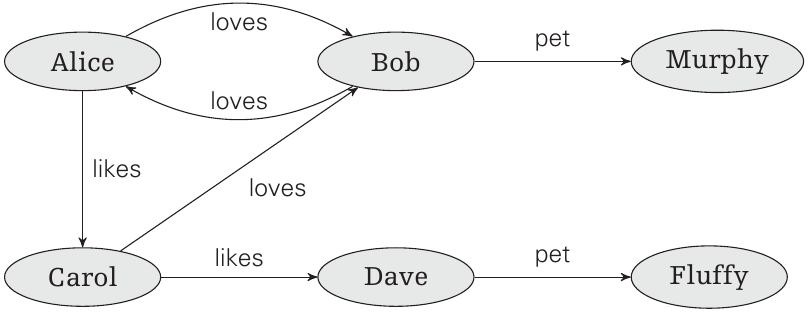
\includegraphics[scale=0.3]{images/graph_example.png}}
\end{frame}


\begin{frame}{Строковые языки запросов}
  \begin{itemize}
    \item Для запросов к графам используются строковые языки запросов, например, Cypher для Neo4j
    \item Отсутствие проверки корректности запроса на этапе компиляции
    \item Невозможность задать контекстно-свободные ограничения
  \end{itemize}
\end{frame}


\begin{frame}[fragile]{Парсер-комбинаторы}
  \begin{itemize}
    \item Парсер-комбинаторы - функции высшего порядка, определяющие грамматику
    \item Можем объединять комбинаторы последовательно или через альтернативу
    \item Описываем грамматику на языке программирования общего назначения
  \end{itemize}


  \begin{minted}[frame=single,framesep=10pt]{kotlin}
val s1 = "A".p seq "B".p
val s2 = "A".p seq "C".p
val s = s1 or s2
  \end{minted}
\end{frame}


\begin{frame}{Применение парсер-комбинаторов к графам}
  \begin{itemize}
    \item Парсер-комбинатор может описывать ограничения на пути в графе
    \item Можем описать предикаты на вершины, исходящие ребра и т.д.
    \item Можем скомбинировать парсеры для поиска определенных путей или циклов
    \item На выходе получаем ноль или более путей. Путей может быть бесконечно много
  \end{itemize}
\end{frame}

\begin{frame}{Trails}
  Trails - библиотека парсер-комбинаторов для запросов к графам.
  \begin{itemize}
    \item Преимущества:
          \begin{itemize}
            \item Прост в использовании
            \item Типизация контролирует корректность парсера
          \end{itemize}
          \vspace{0.5cm}
    \item Недостатки:
          \begin{itemize}
            \item Не поддерживает леворекурсивные грамматики
            \item Имеет ограниченную поддержку циклов
            \item Экспоненциальная сложность
          \end{itemize}
  \end{itemize}
\end{frame}

\begin{frame}{Meerkat}
  Meerkat - изначально библиотека с комбинаторами для разбора текста, реализующий алгоритм из статьи \footnote{\href{https://dl.acm.org/doi/10.1145/2847538.2847539}
    {Izmaylova et al (2016). Practical, General Parser Combinators}}, в последствии расширена поддержкой запросов к графам.
  \begin{itemize}
    \item Преимущества:
          \begin{itemize}
            \item Поддерживает леворекурсивные грамматики и циклы в графе
            \item Имеет сложность $O(n^3)$
          \end{itemize}
          \vspace{0.5cm}
    \item Недостатки:
          \begin{itemize}
            \item Имеет проблемы с типизацией
          \end{itemize}
  \end{itemize}
\end{frame}

\begin{frame}{SPPF}
  \begin{columns}[c]
    \begin{column}{0.5\textwidth}
      SPPF (Shared Packed Parse Forest) -- это структура данных для представления всех возможных разборов в форме леса.
    \end{column}
    \begin{column}{0.55\textwidth}
      \center{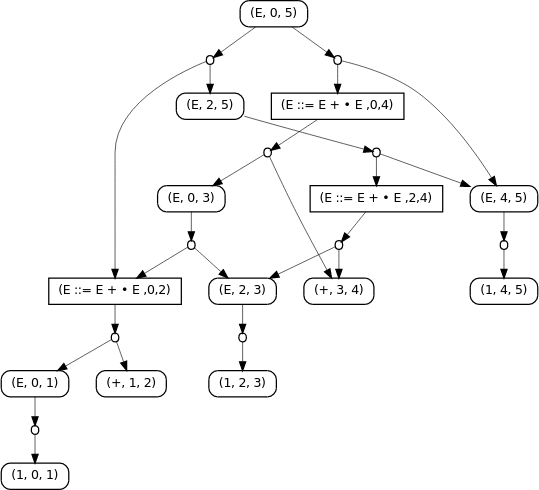
\includegraphics[scale=0.4]{images/sppf_example.png}}
    \end{column}
  \end{columns}
\end{frame}

\begin{frame}{Цель и задачи}
  \textbf{Цель:} Разработать библиотеку комбинаторов запросов к графам на основе алгоритма, предложенного в работе Practical, General Parser Combinators

  \textbf{Задачи:}
  \begin{enumerate}
    \item Разработать базовую структуру парсера и комбинаторов
    \item Поддержать левую рекурсию путем мемоизации результатов парсера
    \item Поддержать циклы, генерируя SPPF дерево
    \item Реализовать извлечение результатов из SPPF дерева
    \item Сравнить скорость работы с другими решениями
  \end{enumerate}
\end{frame}


\begin{frame}[fragile]{Базовая структура парсера}
  \begin{minted}[frame=single,framesep=10pt, fontsize=\small]{kotlin}
Parser<I, O, R>(val inner: (I) -> Sequence<ParserResult<O, R>>)
  \end{minted}
  \begin{itemize}
    \item Базовые комбинаторы: \texttt{seq, or, that, using, many}
    \item Парсеры для графов: \texttt{v, edge, inE, outE, inV, outV}
    \item Определен интерфейс графа, который используют парсеры
  \end{itemize}
  %   \begin{minted}[frame=single,framesep=10pt, fontsize=\small]{kotlin}
  % fun seq(p2: Parser<O, O2, R2>): Parser<In, O2, Pair<R, R2>>
  % fun or(p2: Parser<I, O, R>): Parser<E, I, O, R>
  % fun that(constraint: Parser<O, *, *>): Parser<E, I, O, R>
  % fun using(f: (R) -> R2): Parser<I, O, R2>
  % val Parser<S, S, R>.many: Parser<S, S, Sequence<R>>
  %   \end{minted}
  \begin{minted}[frame=single,framesep=10pt, fontsize=\small]{kotlin}
val person = v()
val mary = outV { it.value == "Mary" }
val loves = outE { it.label == "loves" }
val friend = outE { it.label == "friend" }
val maryLover = person.that(loves seq mary)
val parser = maryLover seq (friend or loves) seq outV()
  \end{minted}
\end{frame}


\begin{frame}[fragile]{Мемоизация результатов}
  \begin{itemize}
    \item Леворекурсивный парсер ($S \to S\ a\ |\ \epsilon$) упадет

    \item Парсер в качестве результата теперь возвращает функцию, принимающую другую функцию (continuation): \mintinline{kotlin}|(Continuation<O, R>) -> Unit|
    \item Continuation будет вызван с результатом вычислений

    \item Парсер мемоизирует результаты для каждого входящего состояния

    \item Результат запоминает все continuations, при появлении нового результата вызывает эти continuations
  \end{itemize}
\end{frame}


\begin{frame}[fragile]{SPPF}
  \begin{itemize}
    \item Парсер графа с циклами потенциально может генерировать бесконечно много результатов
    \item Вместо результатов будем возвращать узлы SPPF дерева
    \item Узлы мемоизируются в процессе парсинга
    \item Узлов конечное количество, поэтому парсинг завершается
  \end{itemize}
\end{frame}


\begin{frame}{Пример SPPF для графа с циклом}
  \begin{columns}
    \begin{column}{0.2\textwidth}
  \raggedleft{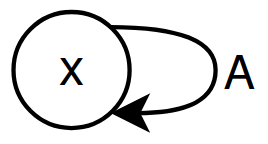
\includegraphics[scale=0.25]{images/graph_loop.png}}
    \end{column}
    \begin{column}{0.8\textwidth}
  \raggedright{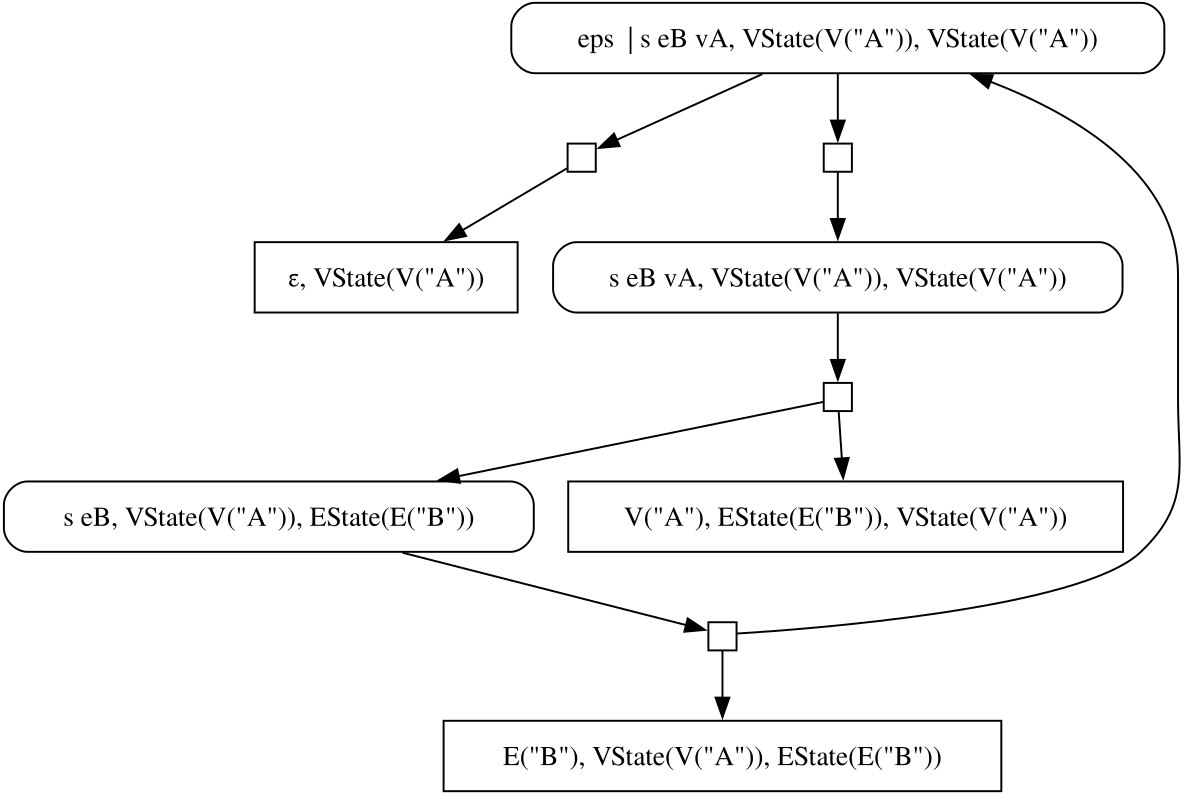
\includegraphics[scale=0.3]{images/sppf_loop.png}}
    \end{column}
  \end{columns}
\end{frame}

\begin{frame}{Извлечение результатов из SPPF}
  \begin{itemize}
    \item Конкретные результаты хранятся в терминальных узлах
    \item Промежуточные узлы объединяют результаты детей либо последовательно, либо через альтернативу
    \item Все вершины могут хранить семантическое действие и применяют его при возврате результата
    \item Дерево обходится в глубину, строя \texttt{Sequence} результатов
  \end{itemize}
\end{frame}


\begin{frame}{Результаты}
  \begin{itemize}
    \item Разработаны базовая структура парсера и комбинаторов, проверяющая корректность во время компиляции
    \item Поддержаны леворекурсивные и неоднозначные грамматики
    \item Поддержаны циклы в графе
    \item Реализована базовая поддержка neo4j графов
  \end{itemize}
\end{frame}


\begin{frame}{В работе}
  \begin{itemize}
    \item Сравнить время работы с другими решениями
    \item Оптимизировать время работы парсеров
  \end{itemize}
\end{frame}


\end{document}

